\documentclass{article}

\usepackage{caption}

\usepackage{enumitem}

\usepackage{graphicx}
\usepackage{float}

\usepackage{amssymb}

\usepackage[
	backend=bibtex,
	sorting=none
]{biblatex}
\addbibresource{refs.bib}

\captionsetup{
	labelfont=bf,
	font=small,
	justification=centering
}
\renewcommand{\figurename}{Fig.}

\title{
	Canning for Amorphous Blob Computing\\
	\small TER report
}

\author{
    Auteur :\\
    Lucas Labouret\\
    M1 QDCS, Université Paris-Saclay\\
    \small lucas.labouret@universite-paris-saclay.fr
    \and
    Encadrant :\\
    Frédéric Gruau\\
    LISN\\
    \small frederic.gruau@universite-paris-saclay.fr
}

\date{}

\begin{document}
 
\maketitle

\begin{figure}[H]
	\centering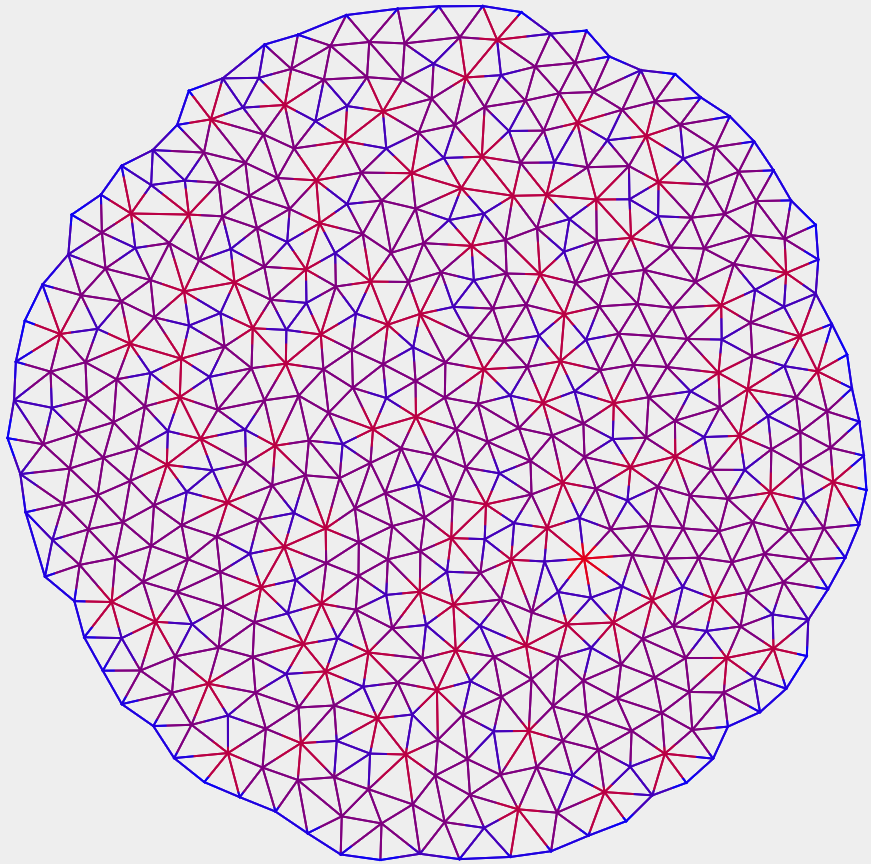
\includegraphics[width=0.9\linewidth]{assets/Circle500.png}
\end{figure}

\newpage
\tableofcontents
\newpage

\renewcommand{\thesection}{\Alph{section}}

\section{What is blob computing ?}

This TER is part of a long term research project about the concept of "blob computing"\cite{blob_computing}. To understand the exact subject of this TER, it is important to first introduce what blob computing means and how it works.\\

The ultimate goal of the project is to develop a new paradigm of computation that is inherently arbitrarily scalable through the use of \textit{space} as a resource. This kind of computation is becoming increasingly useful, for example with the recent development of swarm robotic\cite{swarm_robotic}.

We aim to achieve this through the use of arbitrarily many processing elements (PEs) distributed through space and locally connected. These PEs, which can be severely lacking in power on their own, create a computing medium where virtual "blobs" can form and evolve. These blobs are the main primitive we use for making computations.

\subsection{Definition and structure of a computing medium}

\begin{figure}[H]
	\centering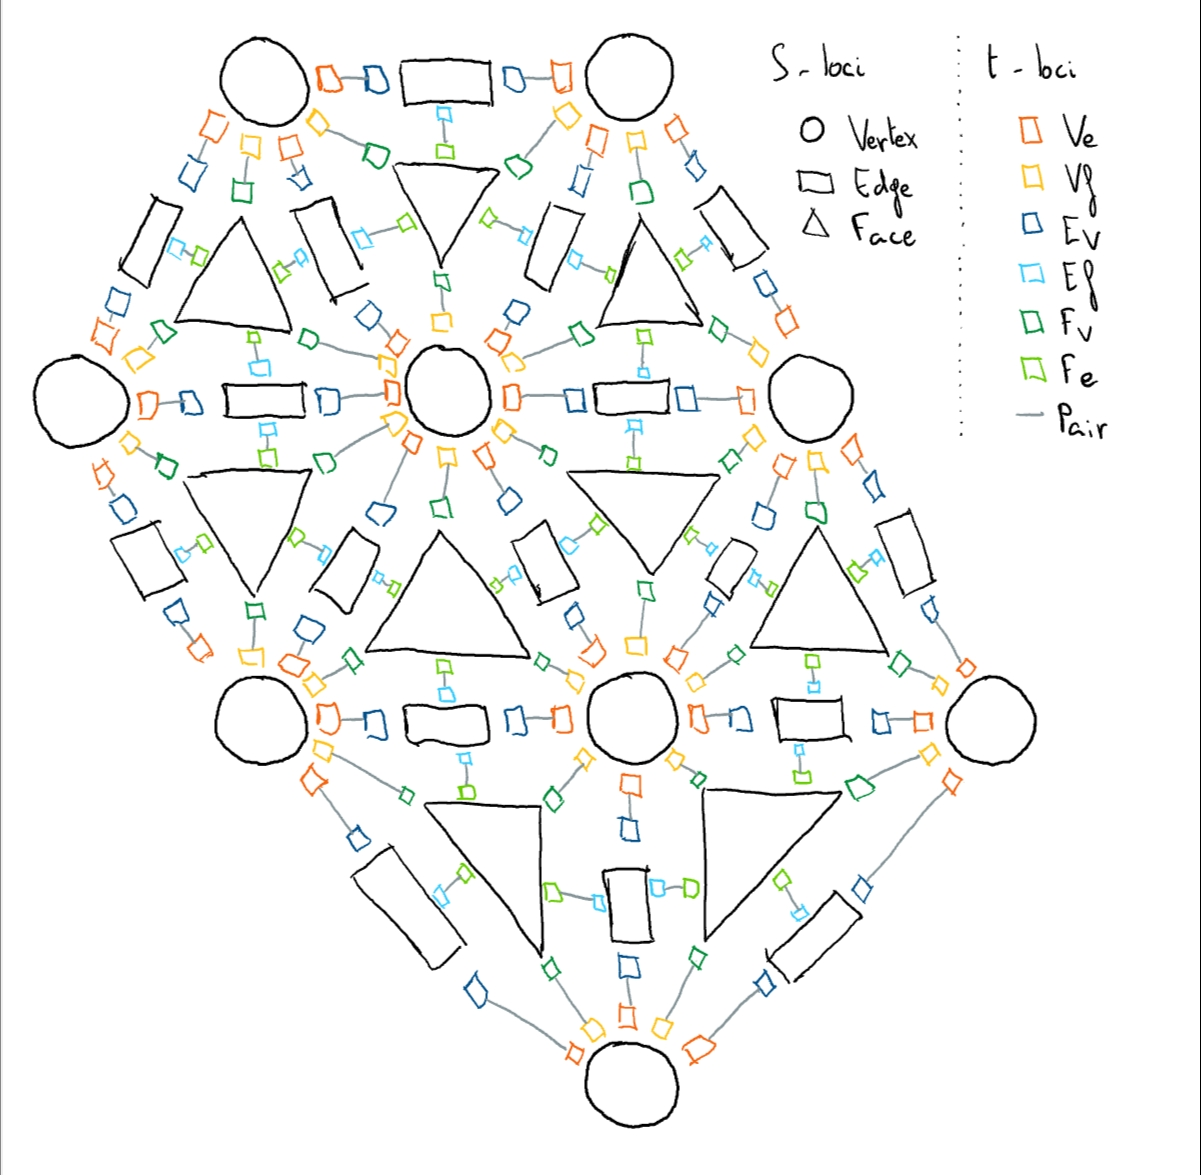
\includegraphics[width=0.9\linewidth]{assets/handdrawn_medium.png}
	\caption{Example structure of a medium.}
	\label{fig:example_structure}
\end{figure}

A computing medium is a weakly Delaunay-triangulated planar graph where each vertex, edge, and face is associated with a processing element capable of executing minimal computation, storing information, and communicating with its neighbors.

Vertices, edges and faces are called "simplicial loci" (or "S-loci" for short). They determine the overall structure of their medium. Each S-locus controls a set of "transfer loci" (or "t-loci"). T-loci come in pairs that handle the communication between two S-loci. For example, if a vertex was connected to an edge, there would be a pair of t-loci (one belonging to the vertex and the other belonging to the edge) between them.

Obviously, there are 3 types of S-loci : Vertex, Edge, Face. T-loci are divided into 6 types : 
\begin{itemize}[noitemsep,nosep]
	\item Ve linking a  Vertex to an Edge
	\item Vf linking a  Vertex to a  Face
	\item Ev linking an Edge   to a  Vertex
	\item Ef linking an Edge   to a  Face
	\item Fv linking a  Face   to a  Vertex
	\item Fe linking a  Face   to an Edge
\end{itemize}
Figure~\ref{fig:example_structure} show an example of how all these loci are put together to form a medium.

A medium is said to be crystalline if a repeating structure emerges in the placement if its vertices. It is amorphous when no such structure emerges. Additionally, it is homogeneous if the average point density is approximately constant and there are no
“holes” or “clusters”, and it is isotropic if the directions of the edges of the medium follow a uniform distribution over $[0, \pi[$. This report mainly focuses on amorphous homogeneous isotropic (AHI) media.

\begin{figure}[H]
	\centering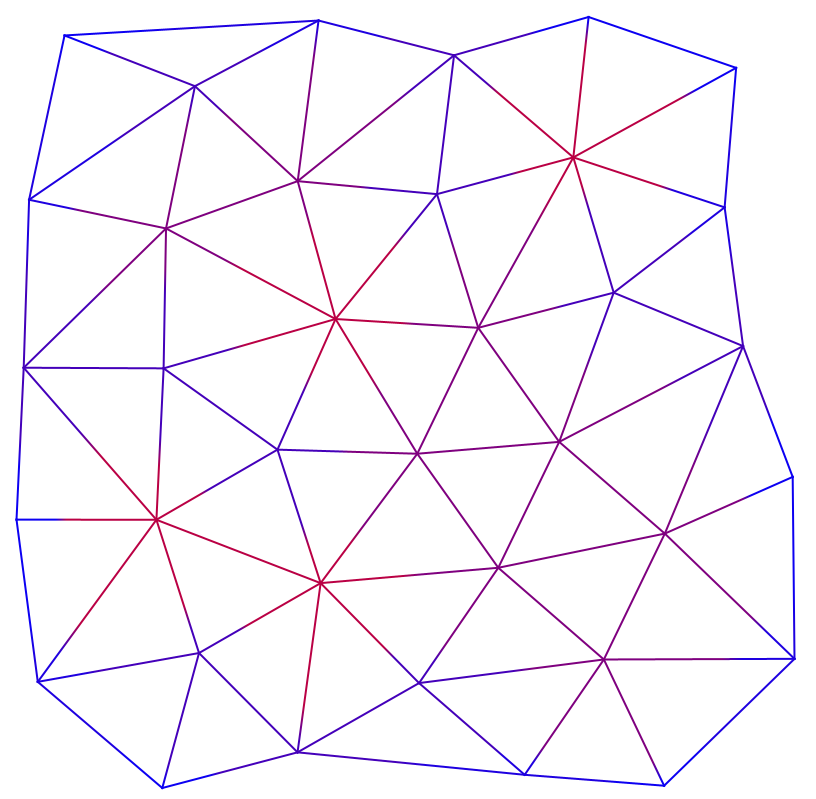
\includegraphics[width=0.4\linewidth]{assets/amorphous_medium.png}
	\hspace{0.1\linewidth}
	\centering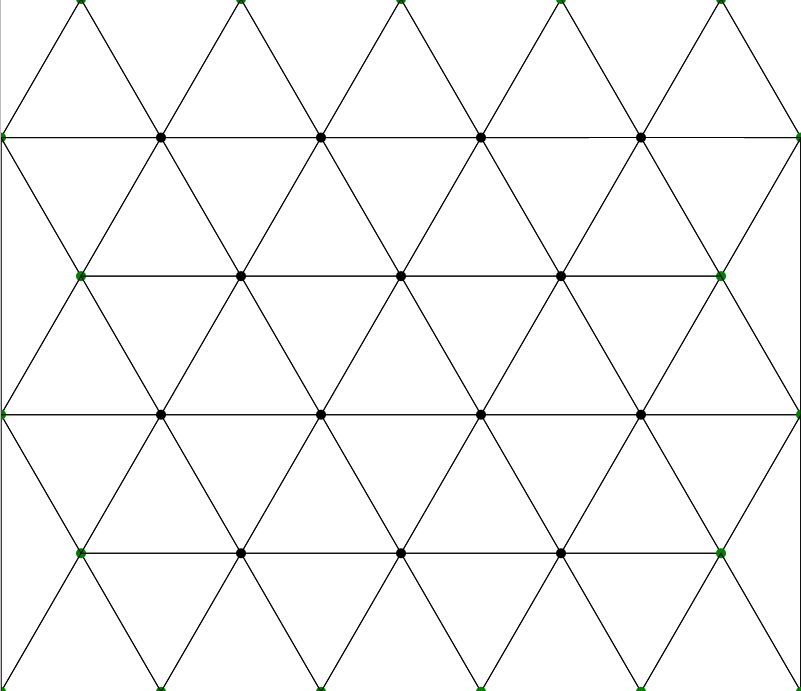
\includegraphics[width=0.4\linewidth]{assets/hexagonal_medium.png}
	\caption{An AHI medium (left) VS a crystalline hexagonal medium (right).}
	\label{fig:amorphous_vs_crystaline}
\end{figure}

For now, we consider PEs to be immobile and synchronous, although lifting these two constraints will probably be the subject of future research.\\

A blob of a given medium $M$ is a connected sub-graph $M'$ of $M$ such that all the vertices of $M'$ share a common property (e.g.: all their values are even, or all their values are 1, etc.). Depending on the program, these blobs are able to grow, shrink, merge, divide and more, which is the computational basis of blob computing.

\subsection{An example of computation : the (discrete) Voronoï diagram}

The article "A parallel data-structure for modular programming of triangulated computing media"\cite{Voronoi} develops tools to program on computing media. As an example, it shows how to build a Voronoï diagram from a set of "seeds" in a medium.

\begin{figure}[H]
	\centering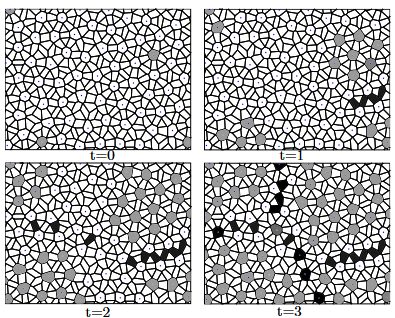
\includegraphics[width=0.7\linewidth]{assets/voronoi_spread.png}
	\caption{
		Computation of a discrete Voronoï diagram.\\
		Cells marked with a dot are the vertices of the medium.
		Gray cells form blobs. Black cells mark the frontiers between blobs. At t=0, blobs only cover the seeds. At t=3, blobs cover the Voronoï regions of the medium.
	}
	\label{fig:voronoi_spread}
\end{figure}

The basic idea is the following : we start with a set of "seeds" distributed over the vertices of the network. Each seed is now the center of a blob. Then, at each synchronous step, the blobs will spread to their adjacent vertices if this wouldn't cause them to merge with another blob, until no blob can spread further. It can be implemented with very few types of local operations that are applied simultaneously to every S-locus in the network :
\begin{itemize}
	\item Multi-cast\\
	The S-locus copies its value into its t-loci of a given type.
	\item Rotation\\
	Since t-loci are spatially arranged around their S-loci, we can define a clockwise and counter-clockwise neighbor. T-loci can perform logical operations on their and their neighbors' values.
	\item Reduction\\
	The S-locus stores the result of a commutative and associative operation applied to the values of its t-loci of a given type.
	\item Transfer\\
	Each of the S-locus' t-loci exchanges its value with the value of its pair. 
\end{itemize}
In fact, clever association of these primitives allows to program everything a computing medium is capable of, such as sorting arrays of integer or multiplying matrices\cite{other_computation}.

\subsection{Objective : Cannings}

Up until now, Gruau mainly focused on hexagonal crystalline media. He built a plateform allowing efficient simulation of blob computation on classical hardware using SIMD\cite{Voronoi}\cite{platform_CA2}. 

The point of this TER is to allow the use of SIMD to optimize the simulation of AHI media as well. We do this through the development of the notion of "canning". Given a medium $M$, a canning is a set of 9 injective maps which assign some integer coordinates to each locus of $M$ :
\begin{enumerate}[noitemsep,nosep]
	\item $\{$Vertex$_M\} \mapsto \mathbb{N}^2$
	\item $\{$Edge$_M\} \mapsto \mathbb{N}^3$
	\item $\{$Face$_M\} \mapsto \mathbb{N}^3$
	\item $\{$Ve$_M\} \mapsto \mathbb{N}^3$
	\item $\{$Vf$_M\} \mapsto \mathbb{N}^3$
	\item $\{$Ev$_M\} \mapsto \mathbb{N}^4$
	\item $\{$Ef$_M\} \mapsto \mathbb{N}^4$
	\item $\{$Fv$_M\} \mapsto \mathbb{N}^4$
	\item $\{$Fe$_M\} \mapsto \mathbb{N}^4$
\end{enumerate}
Through misuse of language, the term "canning" will designate either this set of maps, or the algorithm used to build it.

The objective is twofold : firstly, we want to find a way to measure the efficiency of a canning on a given medium. Secondly, we want to create a canning that is efficient on most -if not all- media.

\section{Preliminary work}

In this section, I detail some work I did last year during another internship with Gruau to generate AHI media. While it isn't the main focus of this year's interniship, it is what made it possible in its current form.

\subsection{Delaunay Triangulation}

\subsection{Farthest Point Optimization}

The Farthest Point Optimization algorithm \cite{FPO} allows for the construction of the irregular yet homogeneous sets of points that we need for blob computing. It yields better results than more common algorithm like Poisson-Disk sampling or Lloyd algorithm, and fits naturally into the project as it relies heavily on the Delaunay triangulation.

The implementation of FPO in my case wasn't straightforward. This is because the article applied the algorithm to sets of points in the unit torus, while the media use bounded subsets of the euclidean plane instead. In particular, I had to adapt the algorithm to work around the existence of borders with no predetermined shape, and that can contain fixed points that cannot be moved even though they can still influence the placement of other points.

\renewcommand{\thesection}{\arabic{section}}
\setcounter{section}{0}

\section{GUI}

A large portion of the TER was focused on the development of a software equipped with a GUI that allows the user to
\begin{enumerate}[noitemsep,nosep]
	\item Randomly generate new media, save them, and load them.
	\item Visualize different aspects of the media.
	\item Compute and visualize different cannings.
\end{enumerate}
$ $

If developing a GUI for this application ended up being time-consuming, it was incredibly helpful all around while debugging everything else. Overall it was probably a net positive on development time alone, and that is still neglecting the advantage of being able to see what i am doing.

\section{Borders and media}

\subsection{Choice of border}

\subsection{Different types of medium}

\section{Canning and evaluation}

\subsection{Partial cannings}

\subsection{Total cannings}

\subsection{Evaluation}

\printbibliography[heading=bibintoc]

\end{document}
